% ============================================================
\section{Results}
\label{sec:results}


% ---------------
%\subsubsection{How successful is the policy at reaching the goal pose?}
\subsection{Success of the policy at reaching the goal pose}
\label{subsec:results_perf}


We evaluate both contact modalities on the same goal-conditioned pushing task and summarize success and terminal errors in Table~\ref{tab:per_family_main_results}. Policies are trained and tested over 500 randomized object variants with diverse initializations and dynamics (Sec.~\ref{subsec:task_protocol}; Table~\ref{tab:domain_rand}). 

% We first focus on in-distribution (ID), which reflects execution quality under the training randomization.

On ID, arm-mediated (AM) pushing achieves higher success and lower terminal errors than whole-body (WB) pushing for both Cuboids and Cylinders. For Cuboids, AM improves success by several points and reduces position error (e.g., $11.64 \rightarrow 8.07$ cm) as well as yaw error ($10.97 \rightarrow 3.85^\circ$). Cylinders show the same trend, with a particularly large reduction in yaw error ($11.75 \rightarrow 3.88^\circ$). Overall, AM’s localized, controllable contact supports finer pose regulation, whereas WB is more sensitive to contact placement on the object. 

% Table~\ref{} provides additional context: under C2, the remaining AM failures on ID are more often yaw-only than position-only, indicating that orientation is the primary limiting factor once the object is near the goal.

% =========================
% TABLE*: per-family main performance (Cuboid + Cylinder)
% =========================
\begin{table*}[t]
\centering
\caption{\textbf{Per-family performance across suites (500 variants).} Results split by object family (Cuboid, Cylinder).}
\label{tab:per_family_main_results}
\footnotesize
\setlength{\tabcolsep}{2.6pt}
\renewcommand{\arraystretch}{1.08}
\begin{tabular}{lcccccccccccccccc}
\toprule
\multirow{3}{*}{\textbf{Suite}} &
\multicolumn{8}{c}{\textbf{Cuboid}} &
\multicolumn{8}{c}{\textbf{Cylinder}} \\
\cmidrule(lr){2-9}\cmidrule(lr){10-17}
& \multicolumn{2}{c}{\textbf{C1 (\%)}} & \multicolumn{2}{c}{\textbf{C2 (\%)}} &
  \multicolumn{2}{c}{\textbf{$e_{\text{pos}}$ cm}} &
  \multicolumn{2}{c}{\textbf{$e_{\psi}$ deg}} &
\multicolumn{2}{c}{\textbf{C1 (\%)}} & \multicolumn{2}{c}{\textbf{C2 (\%)}} &
  \multicolumn{2}{c}{\textbf{$e_{\text{pos}}$ cm}} &
  \multicolumn{2}{c}{\textbf{$e_{\psi}$ deg}} \\
\cmidrule(lr){2-3}\cmidrule(lr){4-5}\cmidrule(lr){6-7}\cmidrule(lr){8-9}
\cmidrule(lr){10-11}\cmidrule(lr){12-13}\cmidrule(lr){14-15}\cmidrule(lr){16-17}
& WB & AM & WB & AM & WB & AM & WB & AM & WB & AM & WB & AM & WB & AM & WB & AM \\
\midrule
ID
& 86.69 & 91.88 & 79.38 & 85.63 & 11.64 & 8.07  & 10.97 & 3.85
& 82.33 & 92.46 & 79.56 & 86.35 &  9.29 & 7.73  & 11.75 & 3.88 \\
OOD-Geometry
& 59.20 & 76.24 & 35.40 & 61.80 & 18.32 & 13.58 & 17.67 & 9.98
& 73.50 & 74.37 & 64.50 & 65.00 & 16.21 & 11.94 & 13.50 & 15.18 \\
OOD-Physics
& 67.50 & 66.87 & 38.12 & 51.88 & 17.46 & 14.34 & 12.63 & 10.39
& 51.00 & 70.00 & 47.50 & 66.87 & 30.83 & 24.86 & 17.28 & 14.71 \\
\bottomrule
\end{tabular}
\vspace{-0.9em}
\end{table*}




%\subsubsection{How does performance generalize under distribution shifts?}
\subsection{Generalization of performance under distribution shifts}
\label{subsec:results_gen}

To evaluate generalization, we test the trained policies on two out-of-distribution suites (OOD-Geometry and OOD-Physics; Sec.~\ref{subsec:task_protocol}) while keeping the task and metrics unchanged (Table~\ref{tab:per_family_main_results}). Both modalities degrade under distribution shift, but the dominant failure modes differ between geometry and physics changes.

\paragraph{OOD-Geometry.}
With novel shapes and aspect ratios, performance drops mainly due to increased sensitivity to contact placement. For \textit{Cuboids}, AM remains markedly stronger: it improves success under both criteria and reduces terminal errors relative to WB. For \textit{Cylinders}, overall success is similar across modalities, but the error profile shifts: AM reduces position error (16.21 $\rightarrow$ 11.94 cm) while exhibiting slightly higher yaw error than WB (13.50 $\rightarrow$ 15.18$^\circ$). This suggests that under geometry shifts, arm contact can still regulate translation effectively, while orientation accuracy can become more sensitive to changes in the effective contact normal.

\paragraph{OOD-Physics.}
When we shift physical properties beyond the training randomization (mass/friction/CoM; Table~\ref{tab:domain_rand}), AM generalizes more reliably than WB. For Cylinders, the gap is larger: AM improves success under both criteria (C1: 70.00 vs.\ 51.00; C2: 66.87 vs.\ 47.50) while reducing both position and yaw errors. This trend is consistent with localized, controllable arm contact helping compensate for physics uncertainty that can destabilize body-based pushing.


\begin{figure}[t]
    \centering
    \includegraphics[width=0.9\linewidth]{Images/Object_Varient.pdf}
    \caption{\textbf{Unseen evaluation objects.} We evaluate the trained policy on 7 chair instances and 5 non-chair objects with diverse geometries.}
    \label{fig:unseen_object_set}
    \vspace{-0.6em}
\end{figure}




\begin{figure}[t]
    \centering
    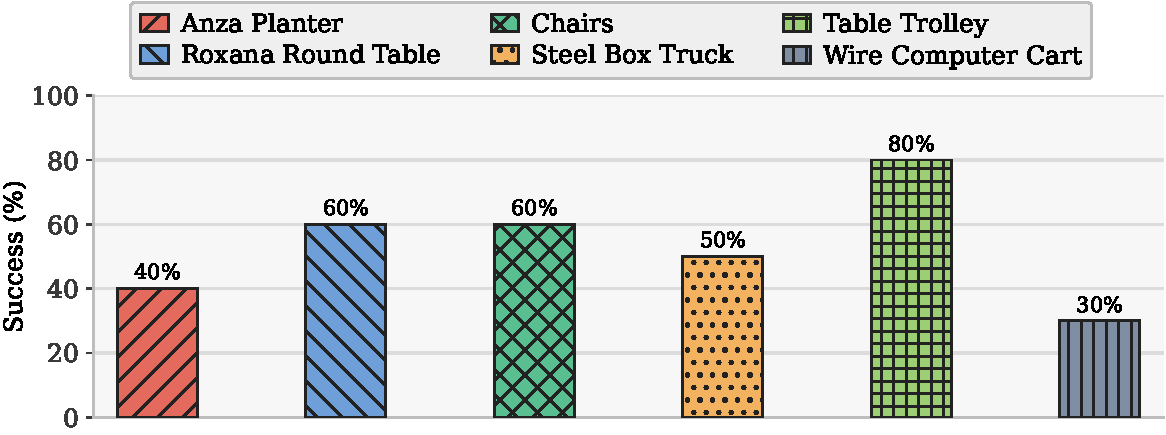
\includegraphics[width=0.75\linewidth]{Images/object_push_success.pdf}
     \caption{\textbf{Success rates on unseen objects.} Category-level success across the evaluation set (Fig.~\ref{fig:unseen_object_set}). Chairs values are average of the 7 Chairs.}
    \label{fig:unseen_object_success}
     \vspace{-0.6em}
\end{figure}

% ---------------
\subsection{Performance generalization across object families}

\label{subsec:results_per_object}


To evaluate whether the learned pushing behavior transfers beyond the parametric Cuboid/Cylinder suites, we test the trained policy on a set of \emph{unseen} everyday objects with diverse shapes and contact affordances. Figure~\ref{fig:unseen_object_set} shows the evaluation set (7 chair instances and 5 other objects), and Fig.~\ref{fig:unseen_object_success} summarizes success across categories. The policy achieves approximately \textit{60\%} average success on unseen chairs, indicating transfer beyond the specific chair instance used during development. Performance drops most noticeably on wheeled objects (e.g., the computer cart), which are outside the training distribution and introduce different interaction dynamics (rolling and reduced sticking) \cite{Scholz2011CartPushing,Mericli2013PushManipulationCasters}. We see a similar failure pattern on the \emph{Anza planter}. Its smooth, continuously curved surface provides fewer stable contact locations and causes the effective contact normal to change rapidly during pushing, which can lead to slip and unintended rotation. Moreover, its near-axisymmetric geometry makes yaw regulation less informative, so small residual rotations can still violate the fixed pose thresholds. Overall, the policy generalizes broadly, with failures concentrated on out-of-distribution contact and mobility.



% ------------------
\paragraph{Interaction footprint}
\label{subsec:results_contact_footprint}

We visualize the policy’s interaction strategy by projecting robot-object contact points onto the object mesh and accumulating a kernelized \emph{interaction footprint}. This provides an interpretable view of \emph{where} the policy prefers to apply contact as training progresses.

Figure~\ref{fig:contact_footprint_train} shows the evolution of this footprint over training checkpoints. Early in training, contacts are %diffuse and 
spread across many regions of the object. Over time, the footprint becomes more structured and concentrated on mechanically effective, repeatable regions, suggesting that the policy learns to consistently exploit favorable contact locations rather than relying on incidental collisions.

% =========================
% FIG: training-time footprint evolution
% =========================
\begin{figure}[t]
    \centering
    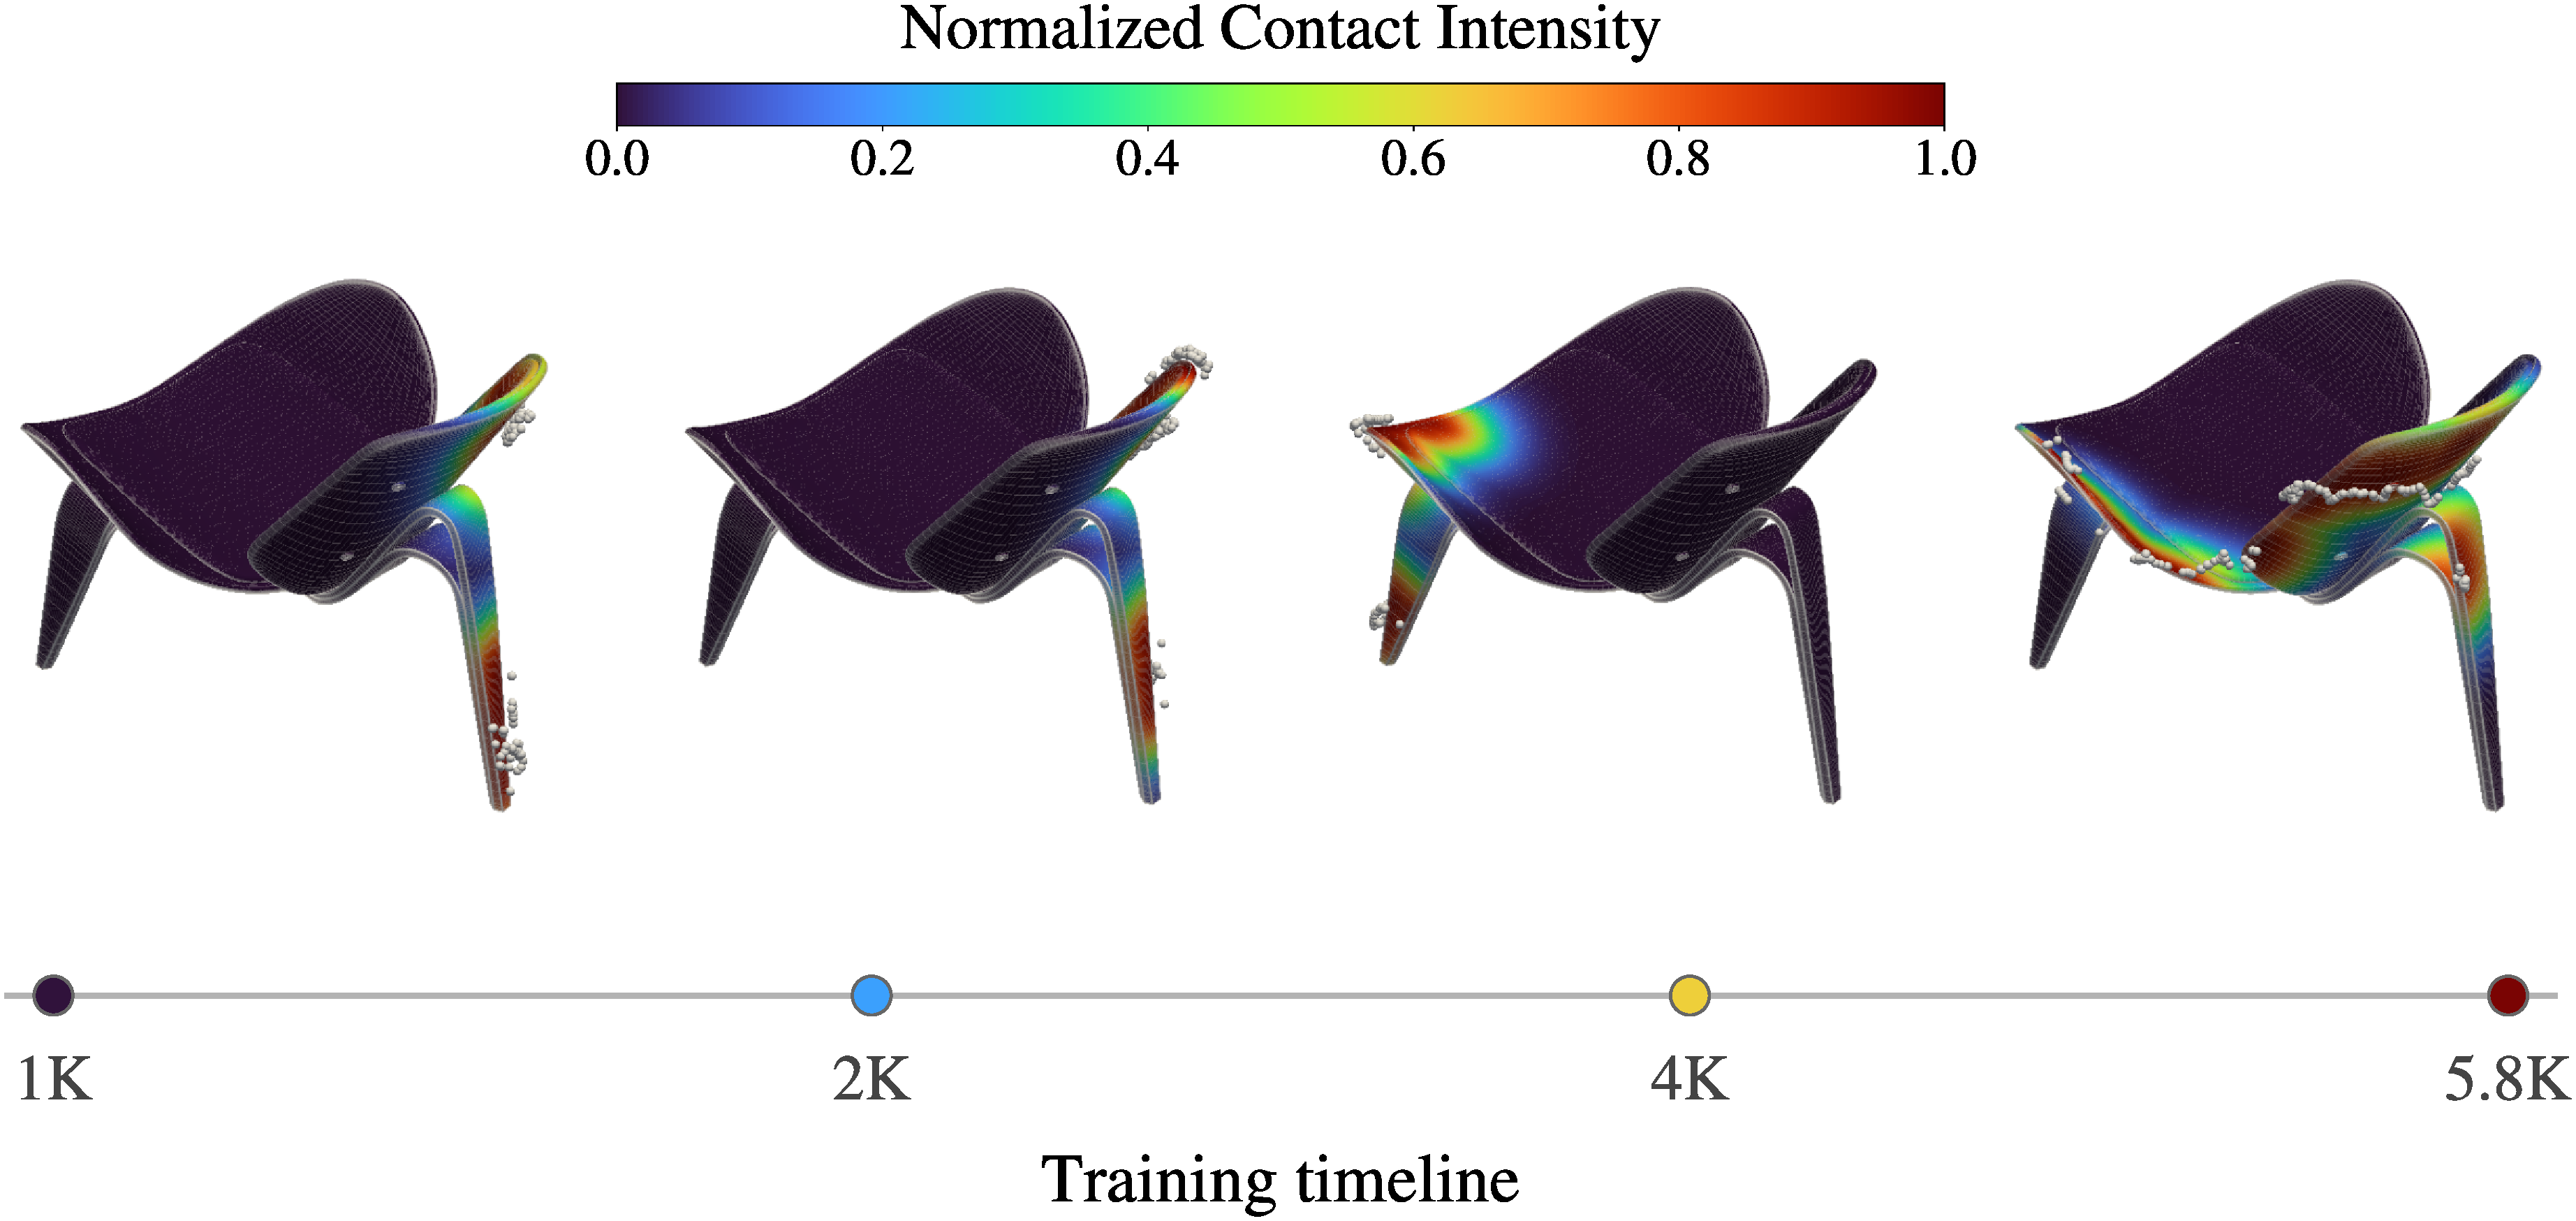
\includegraphics[width= 0.75\linewidth]{Images/checkpoint_heatmaps_timeline_better.pdf}
    \caption{\textbf{Interaction footprint over training.}
    Contact samples projected onto the chair surface across checkpoints. Surface colors show normalized, kernelized contact intensity (higher = more frequent/stronger interaction).}
    \label{fig:contact_footprint_train}
    \vspace{-0.5em}
\end{figure}


% ------------------------------------------------------------
\paragraph{Efficiency in the resulting motion}
\label{subsec:results_efficiency}
We report time-to-success and robot base path length on successful episodes only, and summarize efficiency as goal progress per meter traveled:
\begin{equation}
\label{eq:efficiency_eta}
\eta \triangleq \frac{\max\!\big(0,\ d_{bg}(0)-d_{bg}(T)\big)}{d_{\text{robot}}+\epsilon},
\end{equation}
where $d_{bg}(t)=\|p_o(t)-p_g\|_2$ and $d_{\text{robot}}=\sum_{t=1}^{T}\|p_r(t)-p_r(t-1)\|_2$ is the robot base path length up to success time $T$. As shown in Table~\ref{tab:efficiency}, AM reaches the goal faster and with a substantially shorter base path, yielding higher $\eta$ ($\sim$1.8$\times$ vs.\ WB). Figure~\ref{fig:trajectory_top_view} illustrates this difference on representative rollouts from the same initialization.

% =========================
% TABLE: efficiency
% =========================
\begin{table}[t]
\centering
\caption{\textbf{Efficiency metrics.} Time/path = mean $\pm$ std on successful episodes. $\eta$ = goal progress per meter traveled (higher is better).}
\label{tab:efficiency}
\scriptsize
\setlength{\tabcolsep}{5pt}
\renewcommand{\arraystretch}{1.25}
\begin{tabular}{@{}cccc@{}}
\toprule
\textbf{M} & \textbf{Time (s)} & \textbf{Path (m)} & $\boldsymbol{\eta}$ \\
\midrule
WB & 20.58 $\pm$ 5.92 & 14.99 $\pm$ 3.98 & 0.1058 \\
AM & 10.40 $\pm$ 4.10 & 5.05 $\pm$ 1.76  & 0.1901 \\
\bottomrule
\end{tabular}
\vspace{-0.9em}
\end{table}

\begin{figure}[h]
    \centering
    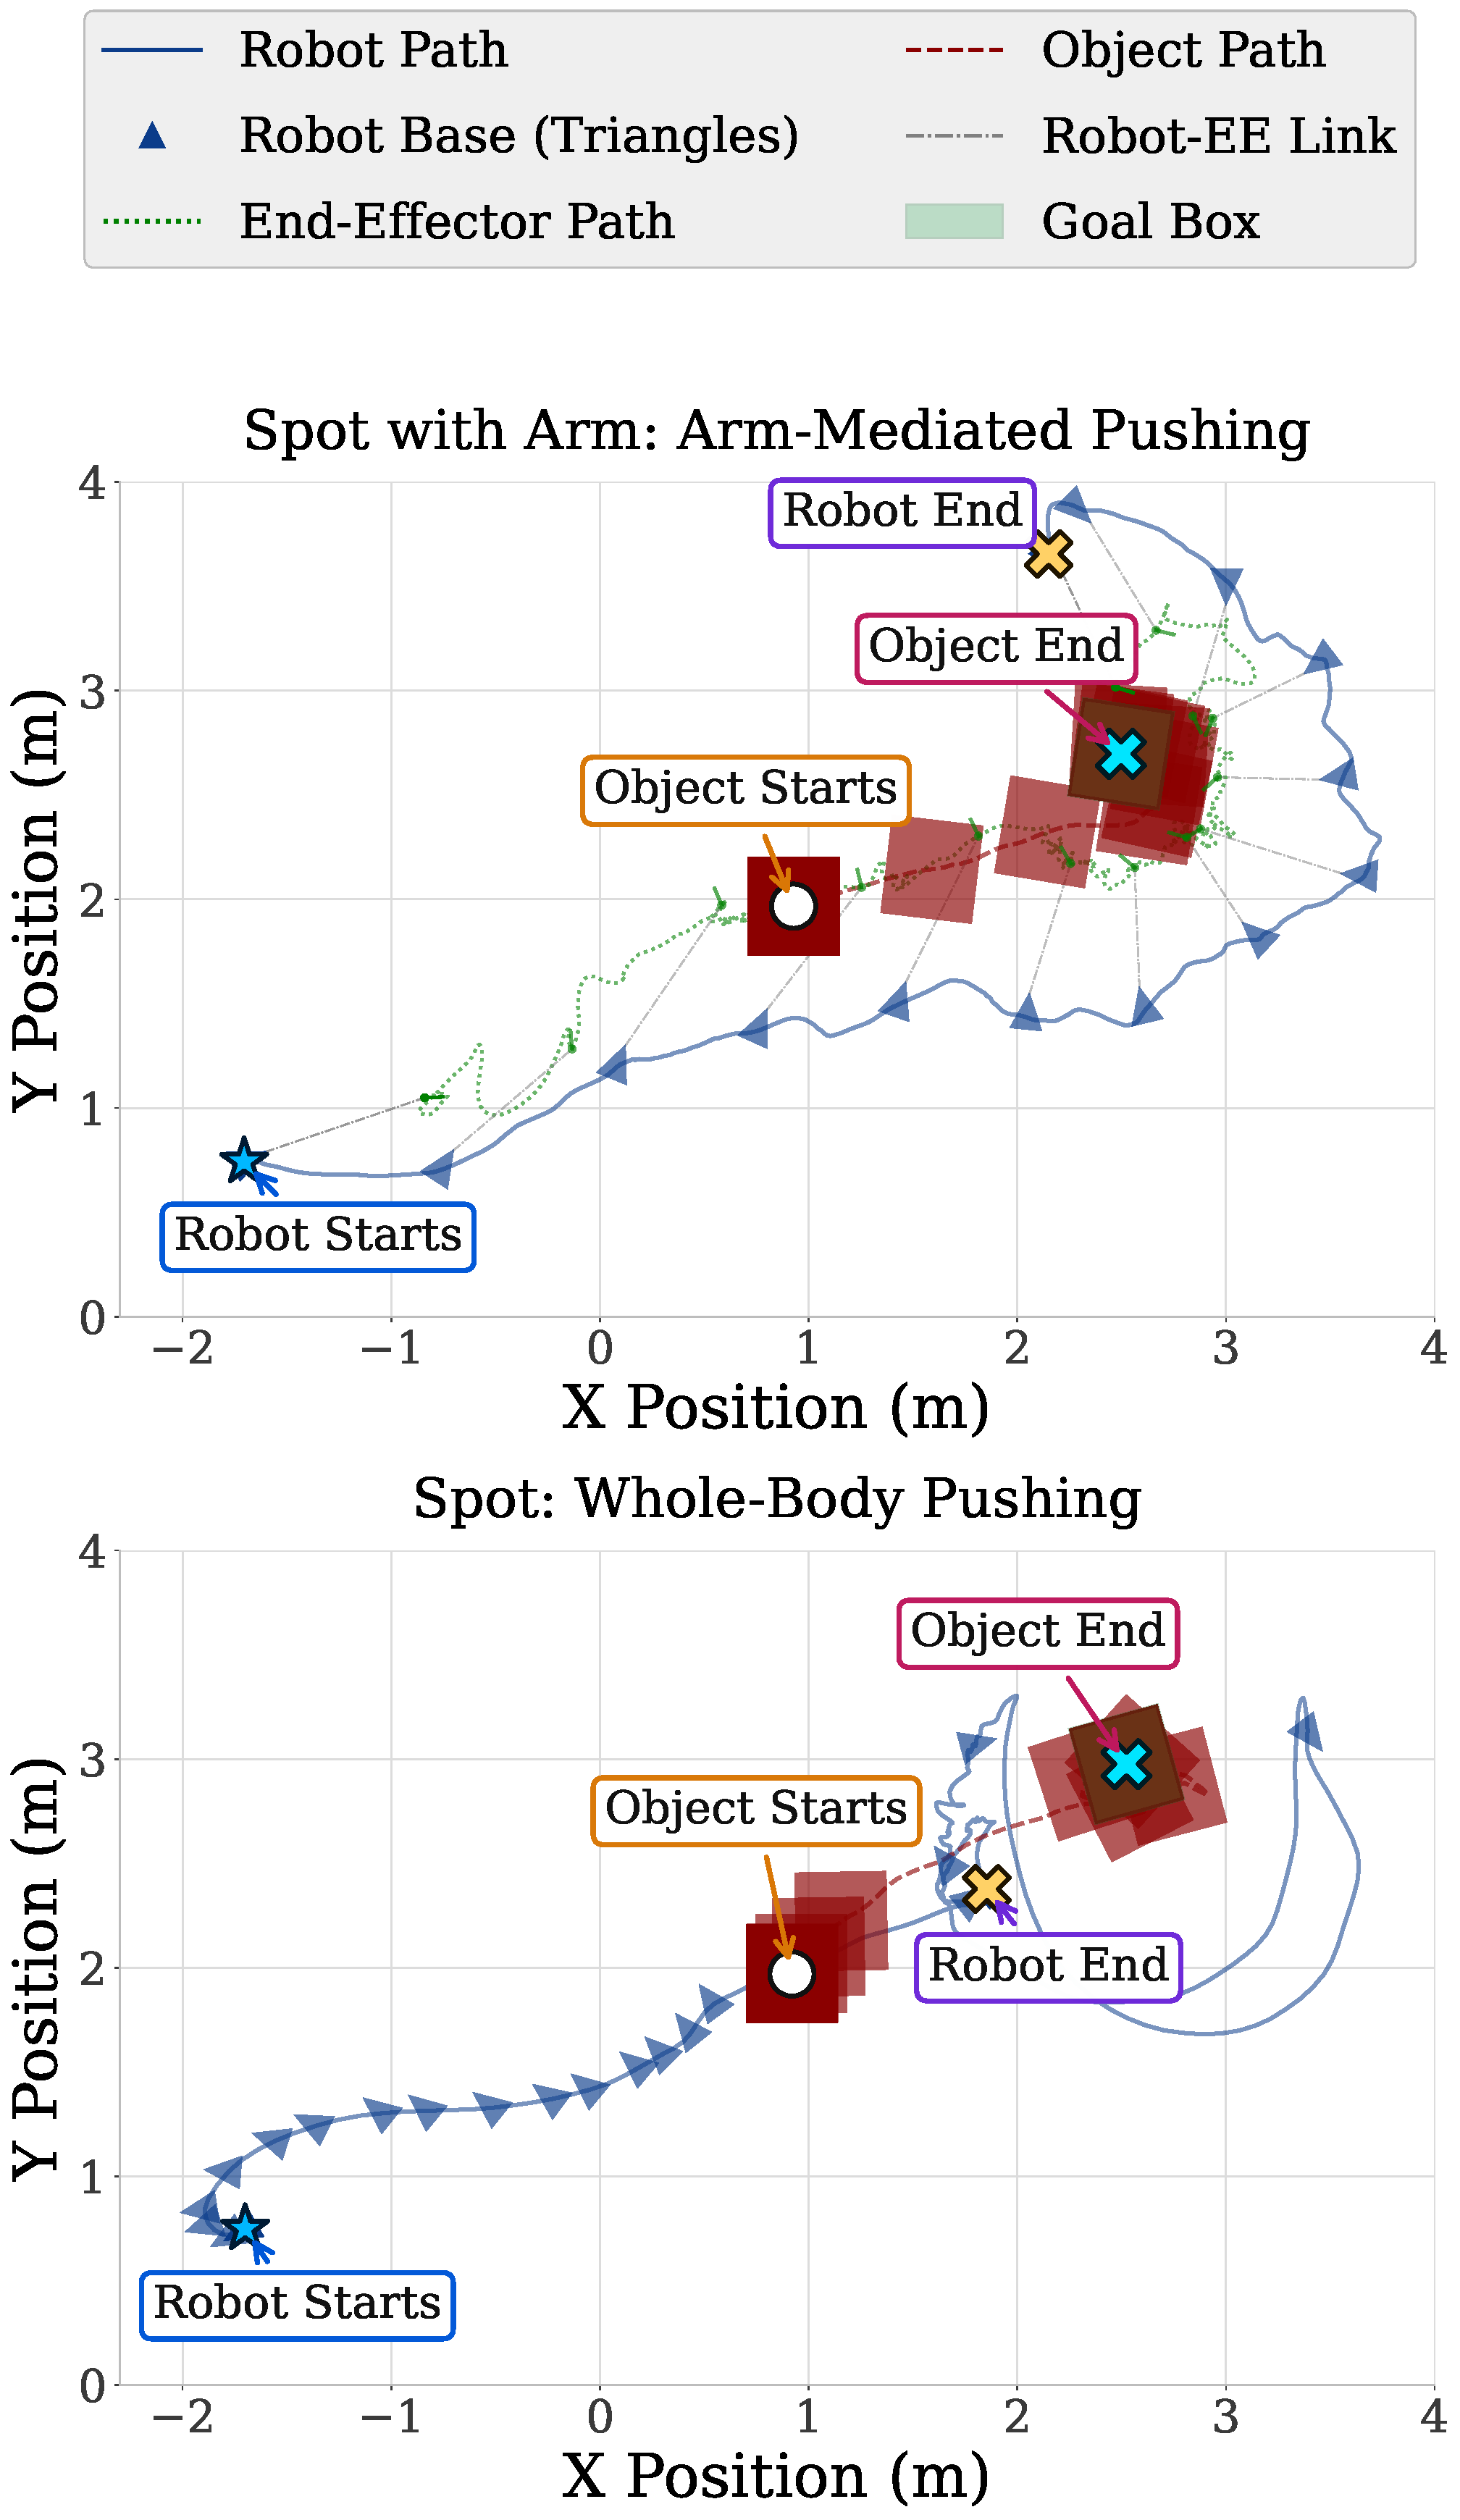
\includegraphics[width=0.8\linewidth]{Images/side_by_side_checkpoints_colored_labels.pdf}
    \caption{\textbf{Top-view rollouts from the same initialization.} Top: AM. Bottom: WB. AM reaches the goal with a shorter base path, while WB typically requires additional base repositioning near the goal.}
    \label{fig:trajectory_top_view}
    \vspace{-0.6em}
\end{figure}


%------------
\paragraph{Ablation study: performance on object unseen during training}
\label{subsec:results_ablation}

To isolate which design choices drive generalization, we performed an ablation study in a cross-chair transfer setting. We train on a single %source 
chair geometry and evaluate on a held-out set of unseen chair geometries. Table~\ref{tab:policy_comparison} summarizes the impact of removing individual components. 
% Removing the reach/sampling signal collapses learning (0\% success), and removing the curriculum severely degrades performance, indicating that guided contact acquisition is necessary for sparse-goal pushing. Removing the encoder also substantially reduces success and increases terminal errors, highlighting the importance of object-conditioned observations for transfer. Our full policy achieves the best performance among non-privileged variants, while an expert policy that directly uses privileged information provides an upper bound.
Eliminating the reward for reaching, which uses point cloud based samples, causes training to collapse (0\% success). This indicates that the shaping term is essential for guiding the agent toward the object and for learning effectively under a sparse-reward signal. Omitting the curriculum for the sparse completion reward term also changes the learned strategy. Arm-mediated pushing degrades into a stiff, base-dominated pushing behavior. We attribute this to reward hacking during early exploration, where the agent discovers easier-to-optimize contacts using the legs or base on different parts of the object instead of establishing purposeful end-effector interactions. Finally, removing the encoder substantially reduces success rates, highlighting its role in embedding exteroceptive observations into a compact latent representation, particularly important for manipulation tasks involving more complex object geometries. Our full policy achieves the best performance among non-privileged variants, while an expert policy that directly uses privileged information provides an upper bound. \footnote{Supplementary materials are available at \url{anonymous-loco-manipulation.github.io}.} 


% =========================
% TABLE*: ablation study
% =========================
\begin{table}[ht]
\centering
\caption{\textbf{Ablation study (train on one chair, test on unseen chairs).} Success reported under Criterion~(C1/C2).}
\label{tab:policy_comparison}
\scriptsize
\setlength{\tabcolsep}{3.2pt}
\renewcommand{\arraystretch}{1.35}
\begin{tabular}{p{4.25cm}cccc}
\toprule
\textbf{Method} & \textbf{C1 (\%)} & \textbf{C2 (\%)} & \textbf{$e_{\text{pos}}$ cm} & \textbf{$e_{\psi}$ deg} \\
\midrule
w/o reach reward (no sampling) & 0.00\% & 0.00\% & N/A & N/A \\
w/o curriculum for sparse reward & 6.25\% & 0.00\% & 184.46 & 77.89 \\
w/o encoder & 39.00\% & 36.91\% & 51.19 & 44.17 \\
Our policy & 69.03\% & 67.64\% & 29.70 & 18.75 \\
Expert policy (privileged inputs) & 79.86\% & 69.51\% & 12.37 & 13.10 \\
\bottomrule
\end{tabular}
\vspace{-0.9em}
\end{table}

% =========================
% FIG: test-time cross-chair transfer
% =========================
% \begin{figure}[t]
%     \centering
%     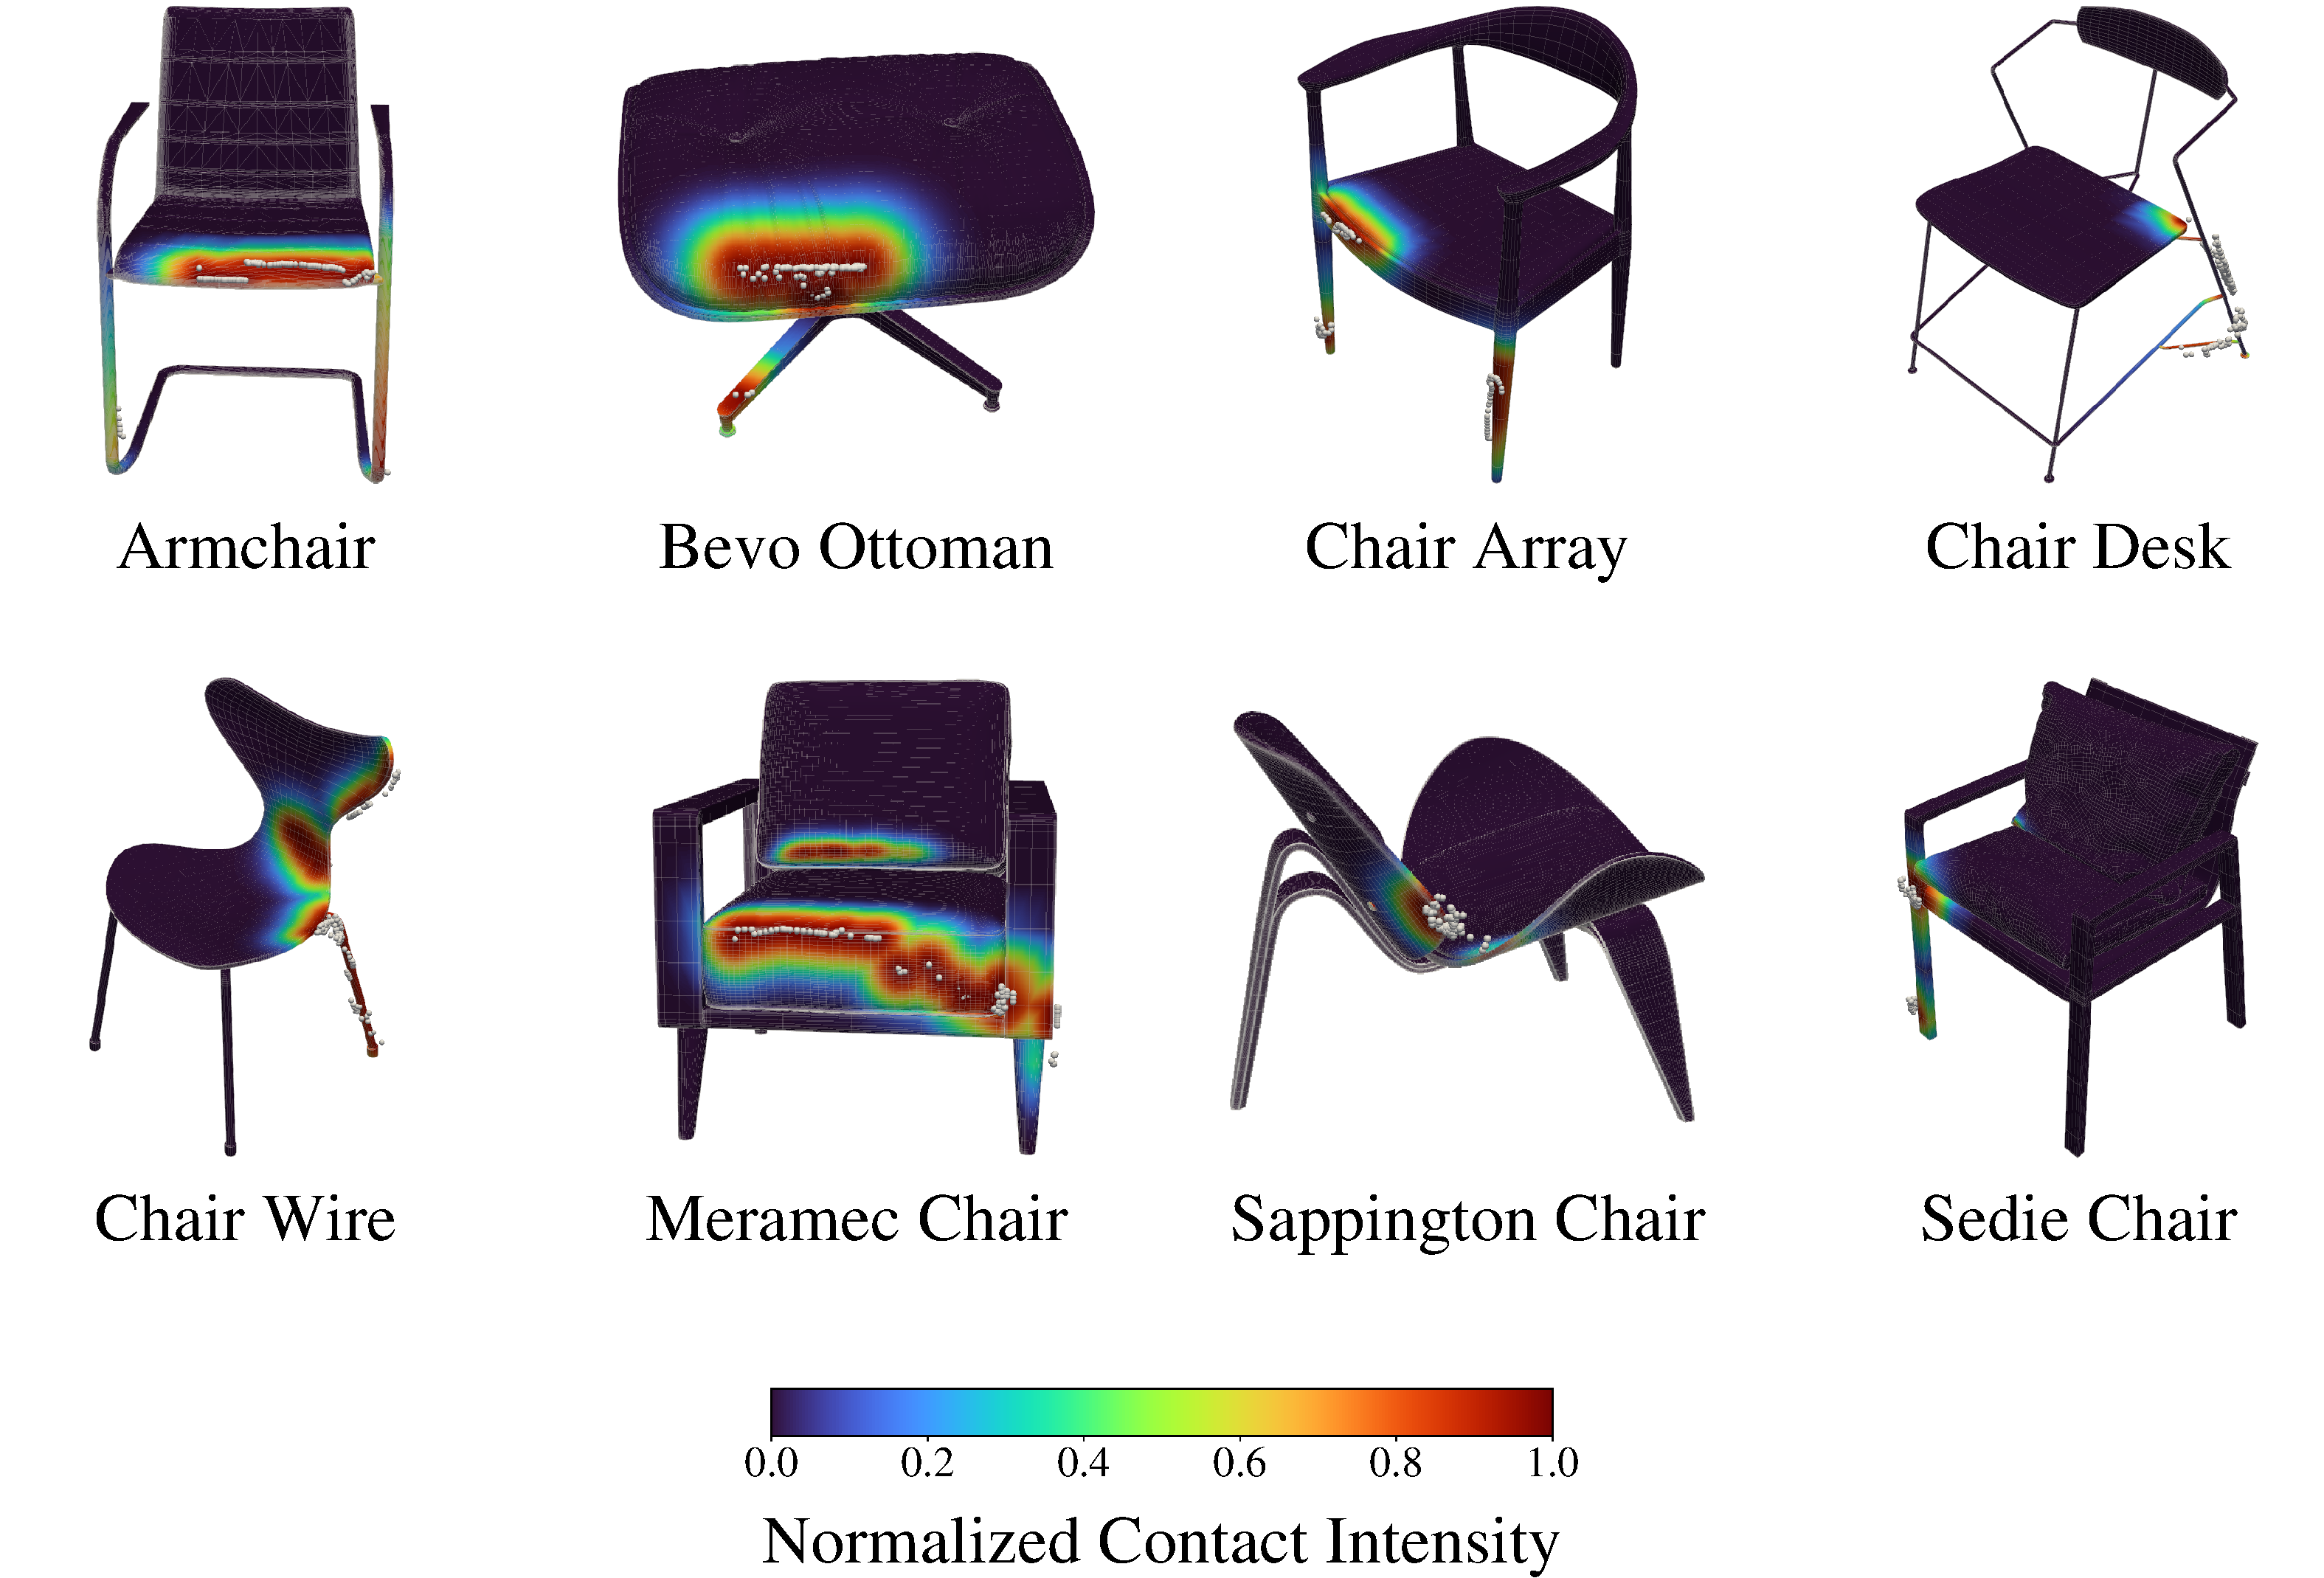
\includegraphics[width=\linewidth]{Images/chair_heatmaps_group_4col_landscape.pdf}
%     \caption{\textbf{Test-time cross-chair transfer}.
%     Each panel shows a rollout on a different chair geometry with the same policy. Markers denote contact samples; surface colors show normalized cumulative contact frequency.}
%     \label{fig:contact_heatmaps_transfer}
%     \vspace{-0.9em}
% \end{figure}

% \noindent\textbf{Takeaway.}
% The timeline supports that learning progresses from diffuse exploration to structured, repeatable contact.
% Cross-chair heatmaps support that the policy transfers contact strategy across geometry rather than memorizing a single mesh.



% \paragraph{Learning curves.}
% % \noindent\textit{How we evaluate.}
% We track optimization progress and interpretability by logging total reward alongside task-grounded errors ($e_{\text{pos}}, e_{\psi}$) during training.

% Figure~\ref{fig:learning_curves} reports total reward, object-goal position error, and object-goal orientation error over iterations.

% % =========================
% % FIG: learning curves
% % =========================
% \begin{figure}[ht]
%     \centering
%     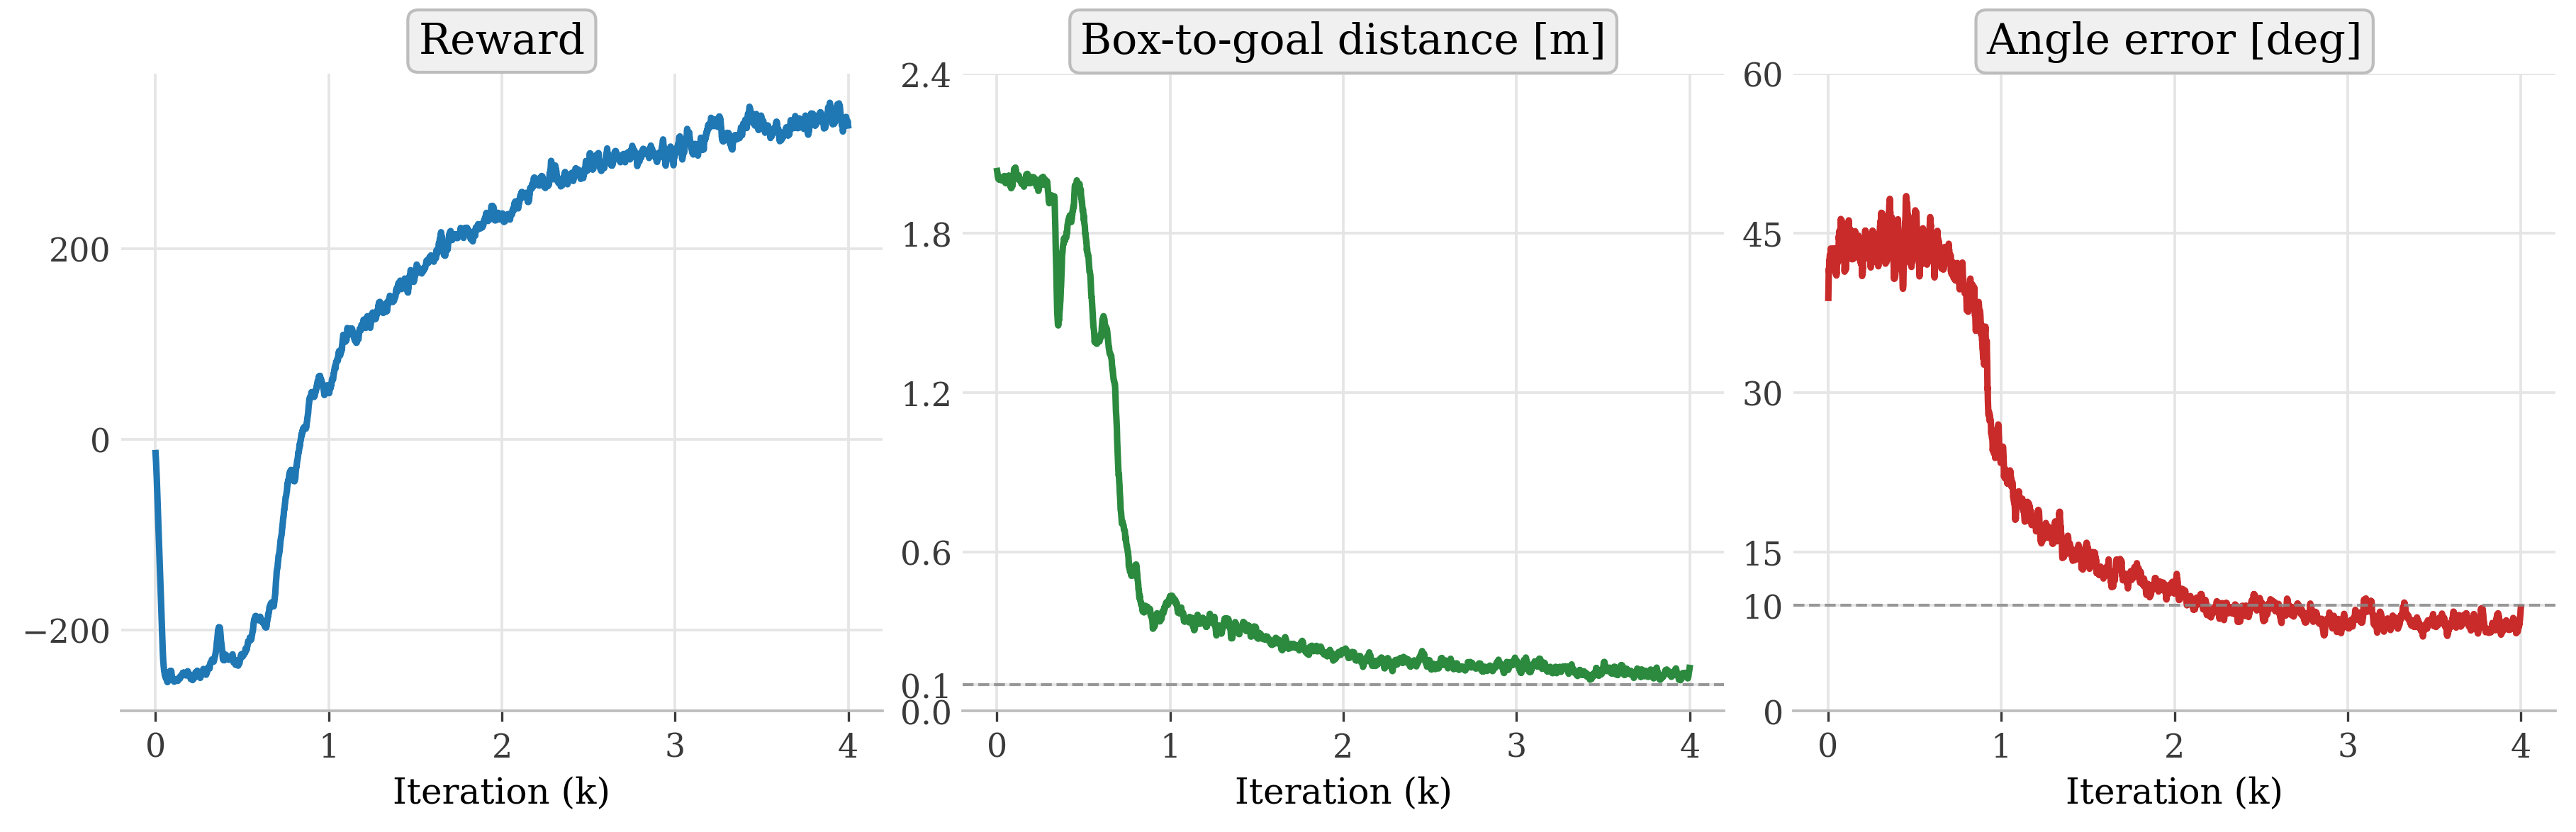
\includegraphics[width=\linewidth]{Images/whole_body_group.png}
%     \caption{\textbf{Learning curves} Training performance over iterations for two control setups. Each grouped figure shows total reward (left), box-to-goal distance error (middle), and angle error (right), with dashed reference thresholds at 10 cm and 10 degrees for error metrics.}
%     \label{fig:learning_curves}
%     \vspace{-0.9em}
% \end{figure}



% % \noindent\textbf{Takeaway.}
% % Reporting reward together with task-grounded errors helps verify that learning corresponds to real progress (reducing pose error), rather than exploiting reward shaping artifacts.


% \begin{table*}[ht]
% \centering
% \caption{\textbf{Ablation Study.}}
% \label{tab:policy_comparison}
% \small
% \setlength{\tabcolsep}{2.6pt}
% \renewcommand{\arraystretch}{1.08}
% \begin{tabular}{lcccc}
% \toprule
% \textbf{Method} & \textbf{Success@15/15} & \textbf{Success@10/10} & \textbf{$e_{\text{pos}}$ cm} & \textbf{$e_{\psi}$ deg} \\
% % & \textbf{(15/15)} & \textbf{(10/10)} & \textbf{(m)} & \\
% \midrule
% w/o reach reward (without sampling) & 0.00\% & 0.00\% & N/A & N/A \\
% w/o curriculum design for sparse reward & 6.25\% & 0.00\% & 184.46 & 77.89 \\
% w/o encoder & 39.00\% & 36.91\% & 51.19 & 44.17 \\
% Our Policy & 69.03\% & 67.64\% & 29.70 & 18.75 \\
% Expert Policy (privileged info direct feeding) & 79.86\% & 69.51\% & 12.37 & 13.10 \\
% \bottomrule
% \end{tabular}
% \vspace{-0.9em}
% \end{table*}




% =========================
% Deployment (sim-to-real)
% =========================
% \subsection{Deployment (sim-to-real)}
% \label{sec:deployment}


% Since we did not have full access to Spot’s integrated whole-body
% loco-manipulation stack due to licensing constraints, we  executed base commands through the Spot API \cite{BostonDynamicsSpotSDK} velocity interface and streamed arm joint targets
% through the arm control API, while preserving the command update rate and safety checks used in simulation (e.g., terminating on loss of stability or unsafe contacts).



